\documentclass[11pt]{article}
\usepackage{geometry}
\geometry{a4paper, left=20mm, top=20mm, right=20mm, bottom=20mm}
\usepackage{fullpage}
\usepackage{amsfonts}
\usepackage{graphicx}

\begin{document}

\title{\textbf{Introduction to Scientific Computing}\\Project Assignment}
\date{\today}
\author{Mikhail Ivanov}
\maketitle

A Python program \texttt{SlabCGBeadMapping.py} that was prepared as the project assignment will be shortly described here.

\section{Motivation and Introduction}

My PhD project is dedicated to the development of coarse-grained molecular models of inorganic materials and biomolecules. In coarse-grained molecular models, one describes not every atom in the molecule, but rather a group of atoms as a single mass point. Using coarse-grained models instead of atomic models for molecular dynamics simulations can drastically reduce the computation times and enable simulations of larger systems on a larger timescale.

Right now I'm working on coarse-grained models of titanium dioxide (TiO\textsubscript{2}) surfaces and phospholipid molecules, which are the main constituents of cell membranes. The first step of developing the coarse-grained model is to decide how to merge atoms inside the molecule. The process of merging atoms into coarse-grained sites, or beads, is usually called \textit{bead mapping}. The bead mapping is rather simple for phospholipid, because one can easily divide the molecule into certain parts that make sense from the chemical point of view. For example, one can introduce a coarse-grained bead that will describe the polar head group of the molecule and another type for the hydrophobic tail groups. The coarse-grained model will contain much fewer sites but will be still amphiphilic (both hydrophilic and hydrophobic) which is a very important property for phospholipids.

It is however not so obvious how to do bead mapping for titanium dioxide surface. Although being a crystalline material, the surface of TiO\textsubscript{2} is quite heterogeneous and contain surface chemical modifications that make the structure irregular.

That is why I wanted to create a general and automatic tool that will do the bead mapping of inorganic surfaces.

\section{Program general workflow}

At the beginning, the program reads atomic coordinates of a rectangular slab. A 3D rectangular user-defined grid is built with the grid points situated inside the slab. The idea is to assign atoms to the grid points in a certain way and use the list of assigned atoms as a bead mapping scheme. The grid points essentially become the future coarse-grained beads.

After reading the atomic coordinates and building the grid, the main part of the program starts - the program first calculates the distances between all atoms and all grid points, sorts the distances and assigns atoms to the nearest grid points.

Since the distribution of atoms within the slab is not completely uniform, the number of assigned atoms to every grid point may differ greatly. This is not very convenient for the coarse-grained model because then one needs to introduce different coarse-grained bead types for grid points with different number of atoms.

So, after all the atoms were assigned to the nearest grid points, the next task for the program is to make the distribution of atoms between the grid points more uniform. To accomplish this, the program goes through every grid point. If the number of assigned atoms is lower than a certain threshold (that is based on the average number of atoms per grid point), than the next-nearest (or \textit{N}-nearest) atom is added to the grid point and removed from another grid point that had the atom before, provided that another grid point has more atoms. It works analogously for the grid points that have a higher number of atoms. The process is repeated for several iterations.

After the distribution is fixed, the indices of the assigned atoms are saved as an output file and the histogram of the distribution is plotted.

Error checking in the program ensures that all the atoms are assigned and no atoms are assigned more than once.

\section{Program structure}

The program is written in Python 3 using \texttt{numpy} library for computations and \texttt{matplotlib} library for plotting the results.

The program consists of four modules:

\begin{enumerate}
\item \texttt{IO.py} - reads atomic coordinates of the system that contains TiO\textsubscript{2} surface
\item \texttt{slabInit.py} - initialize the rectangular grid
\item \texttt{beadMapping.py} - assigns atoms to grid points
\item \texttt{SlabCGBeadMapping.py} - the main module that runs the functions from the other modules
\end{enumerate}

The user can set the name of the file that contains the atomic coordinates, number of grid points along X, Y and Z axes, number of fixing iterations and the neighbor order for reassigning atoms in the main module. 

The program is run with the following command:

\texttt{> python SlabCGBeadMapping.py}

The input file with the used atomic coordinates as well as the resulting bead mapping scheme is provided together with the \texttt{.py} files in the assignment folder.

\section{Results}

The following results are obtained for the coarse-grained bead mapping of 7x7x3 nm anatase (one of the titanium dioxide polymorph) surface slab.

Figure \ref{fig: anatase-101 histogram unfixed} shows the distribution of atoms for the surface CG beads \textbf{before} fixing.

\begin{figure}[h]
\centering
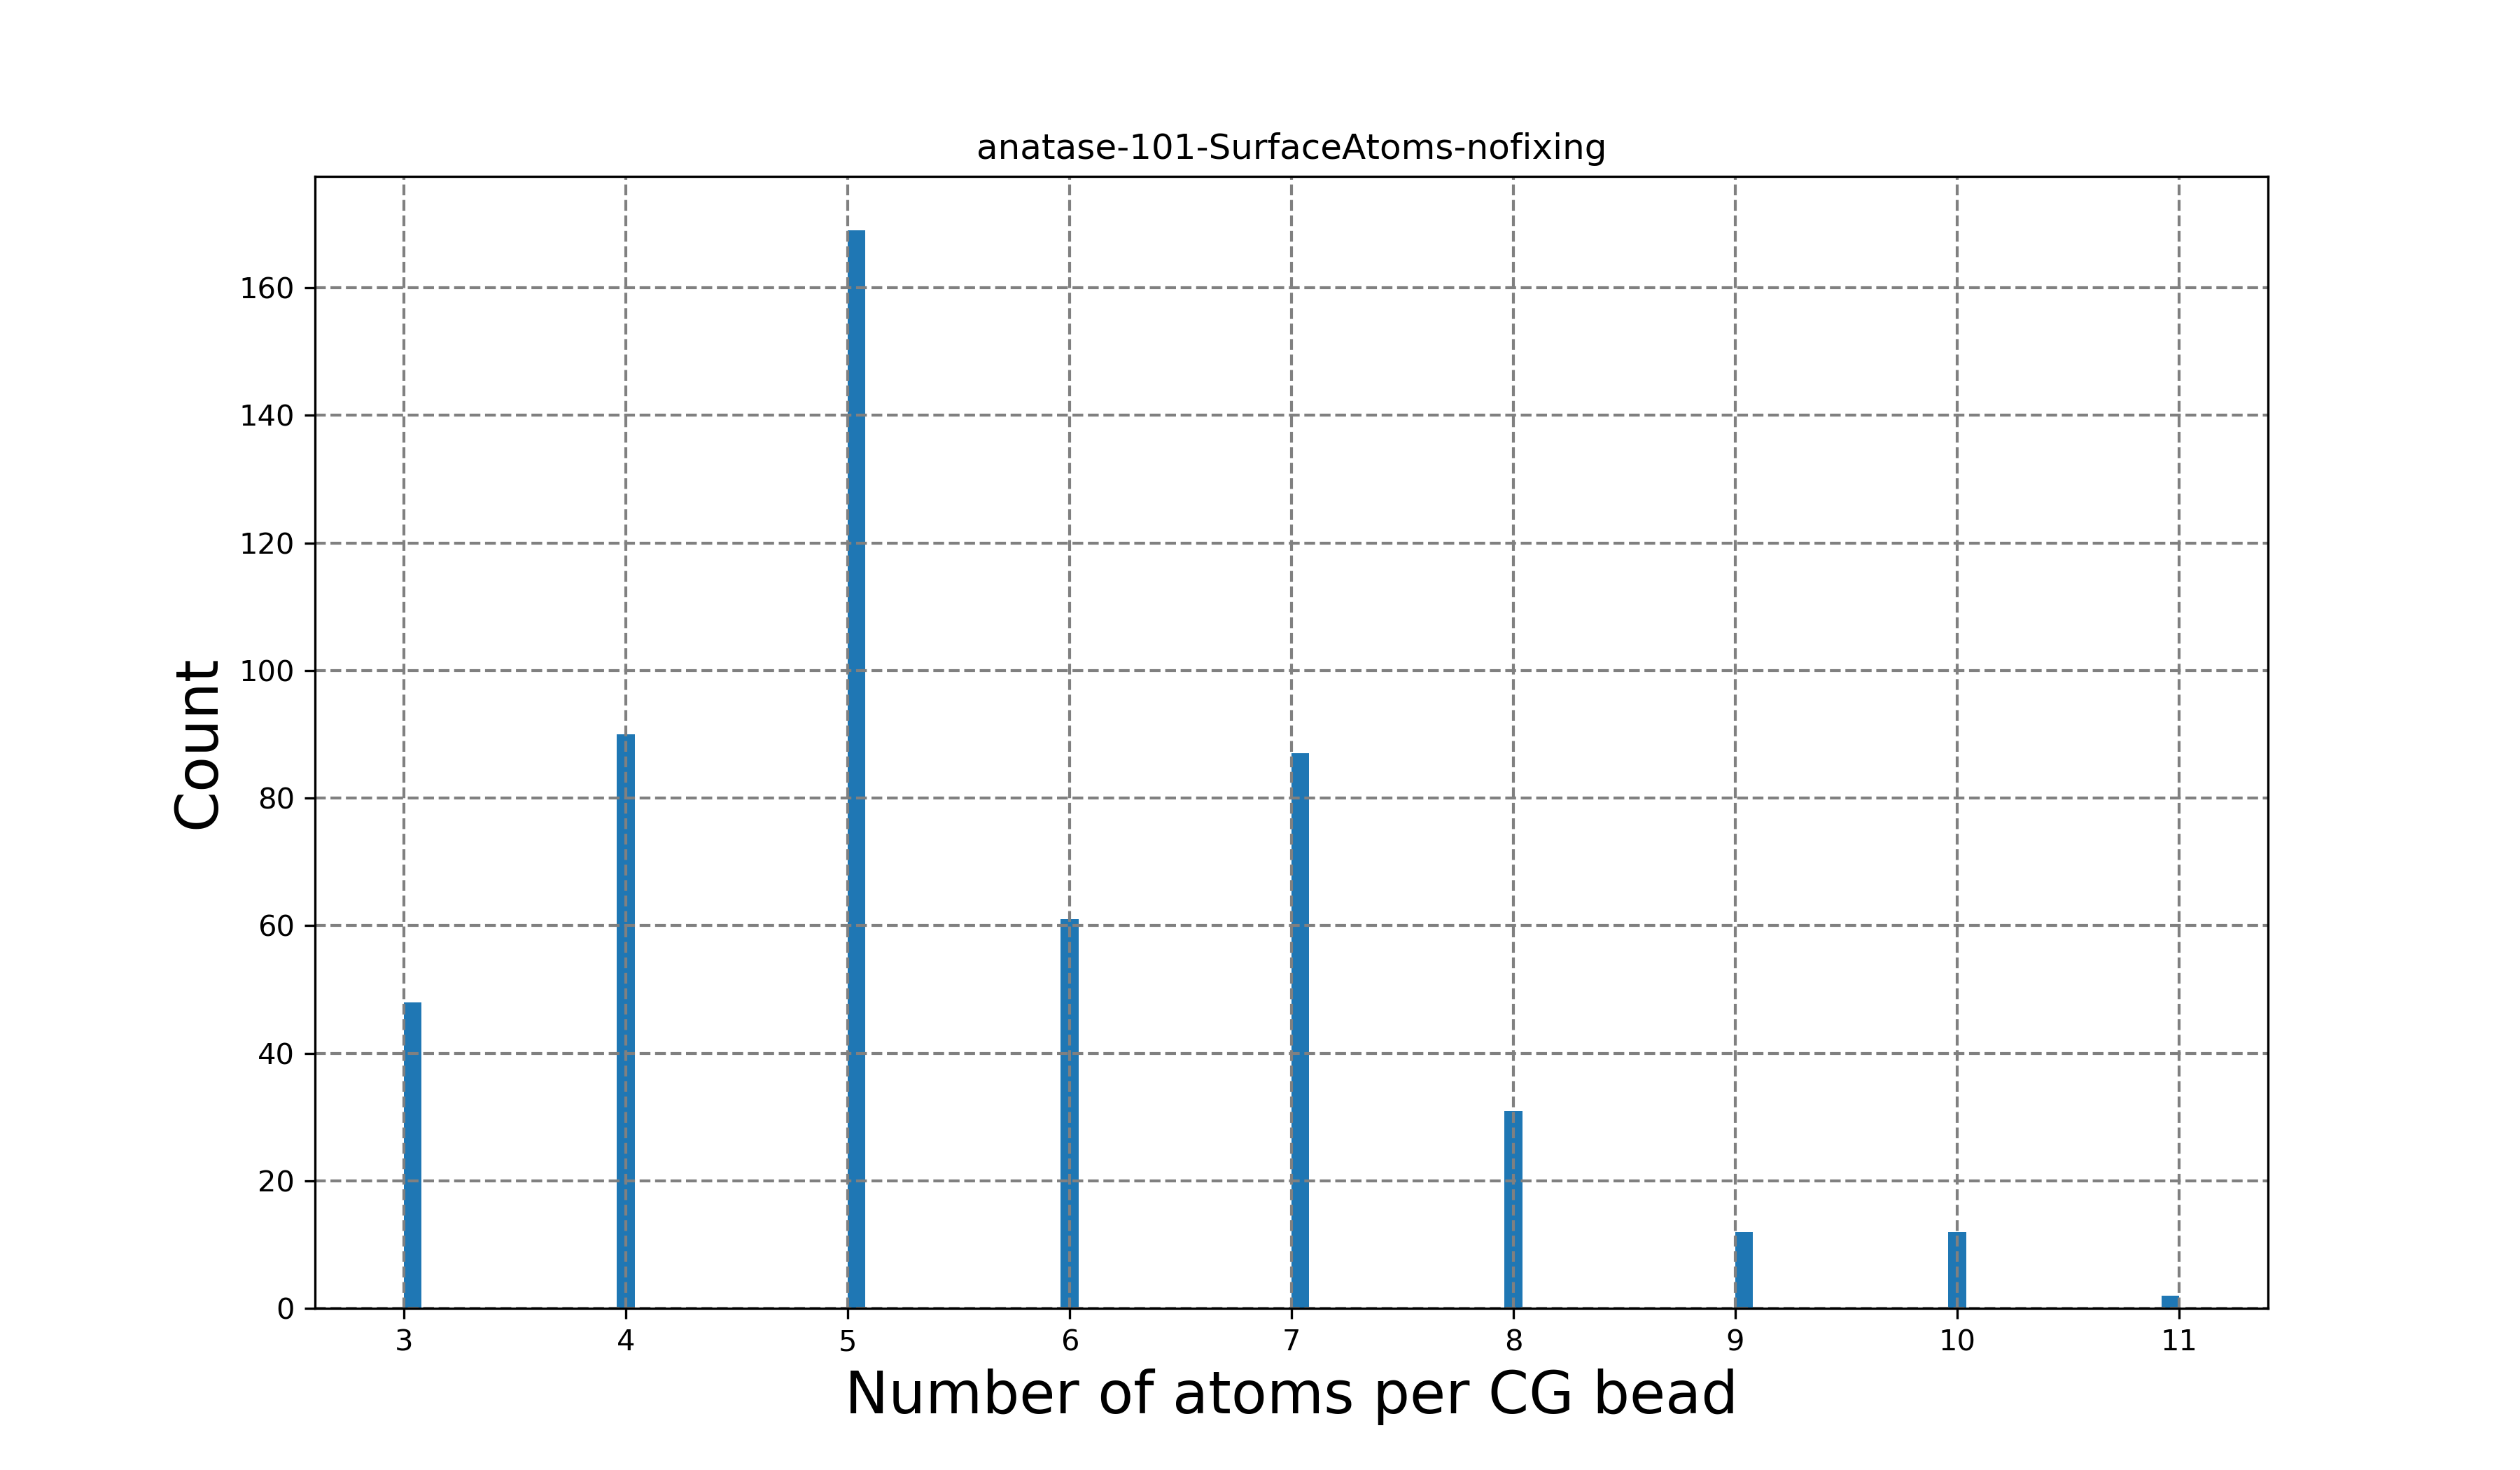
\includegraphics[scale=0.3]{anatase-101-SurfaceAtoms-nofixing.png}
\caption{Distribution of assigned atoms for surface CG beads \textbf{before} fixing.}
\label{fig: anatase-101 histogram unfixed}
\end{figure}

Figure \ref{fig: anatase-101 histogram} shows the distribution of atoms for the surface CG beads \textbf{after} fixing.

\begin{figure}[h]
\centering
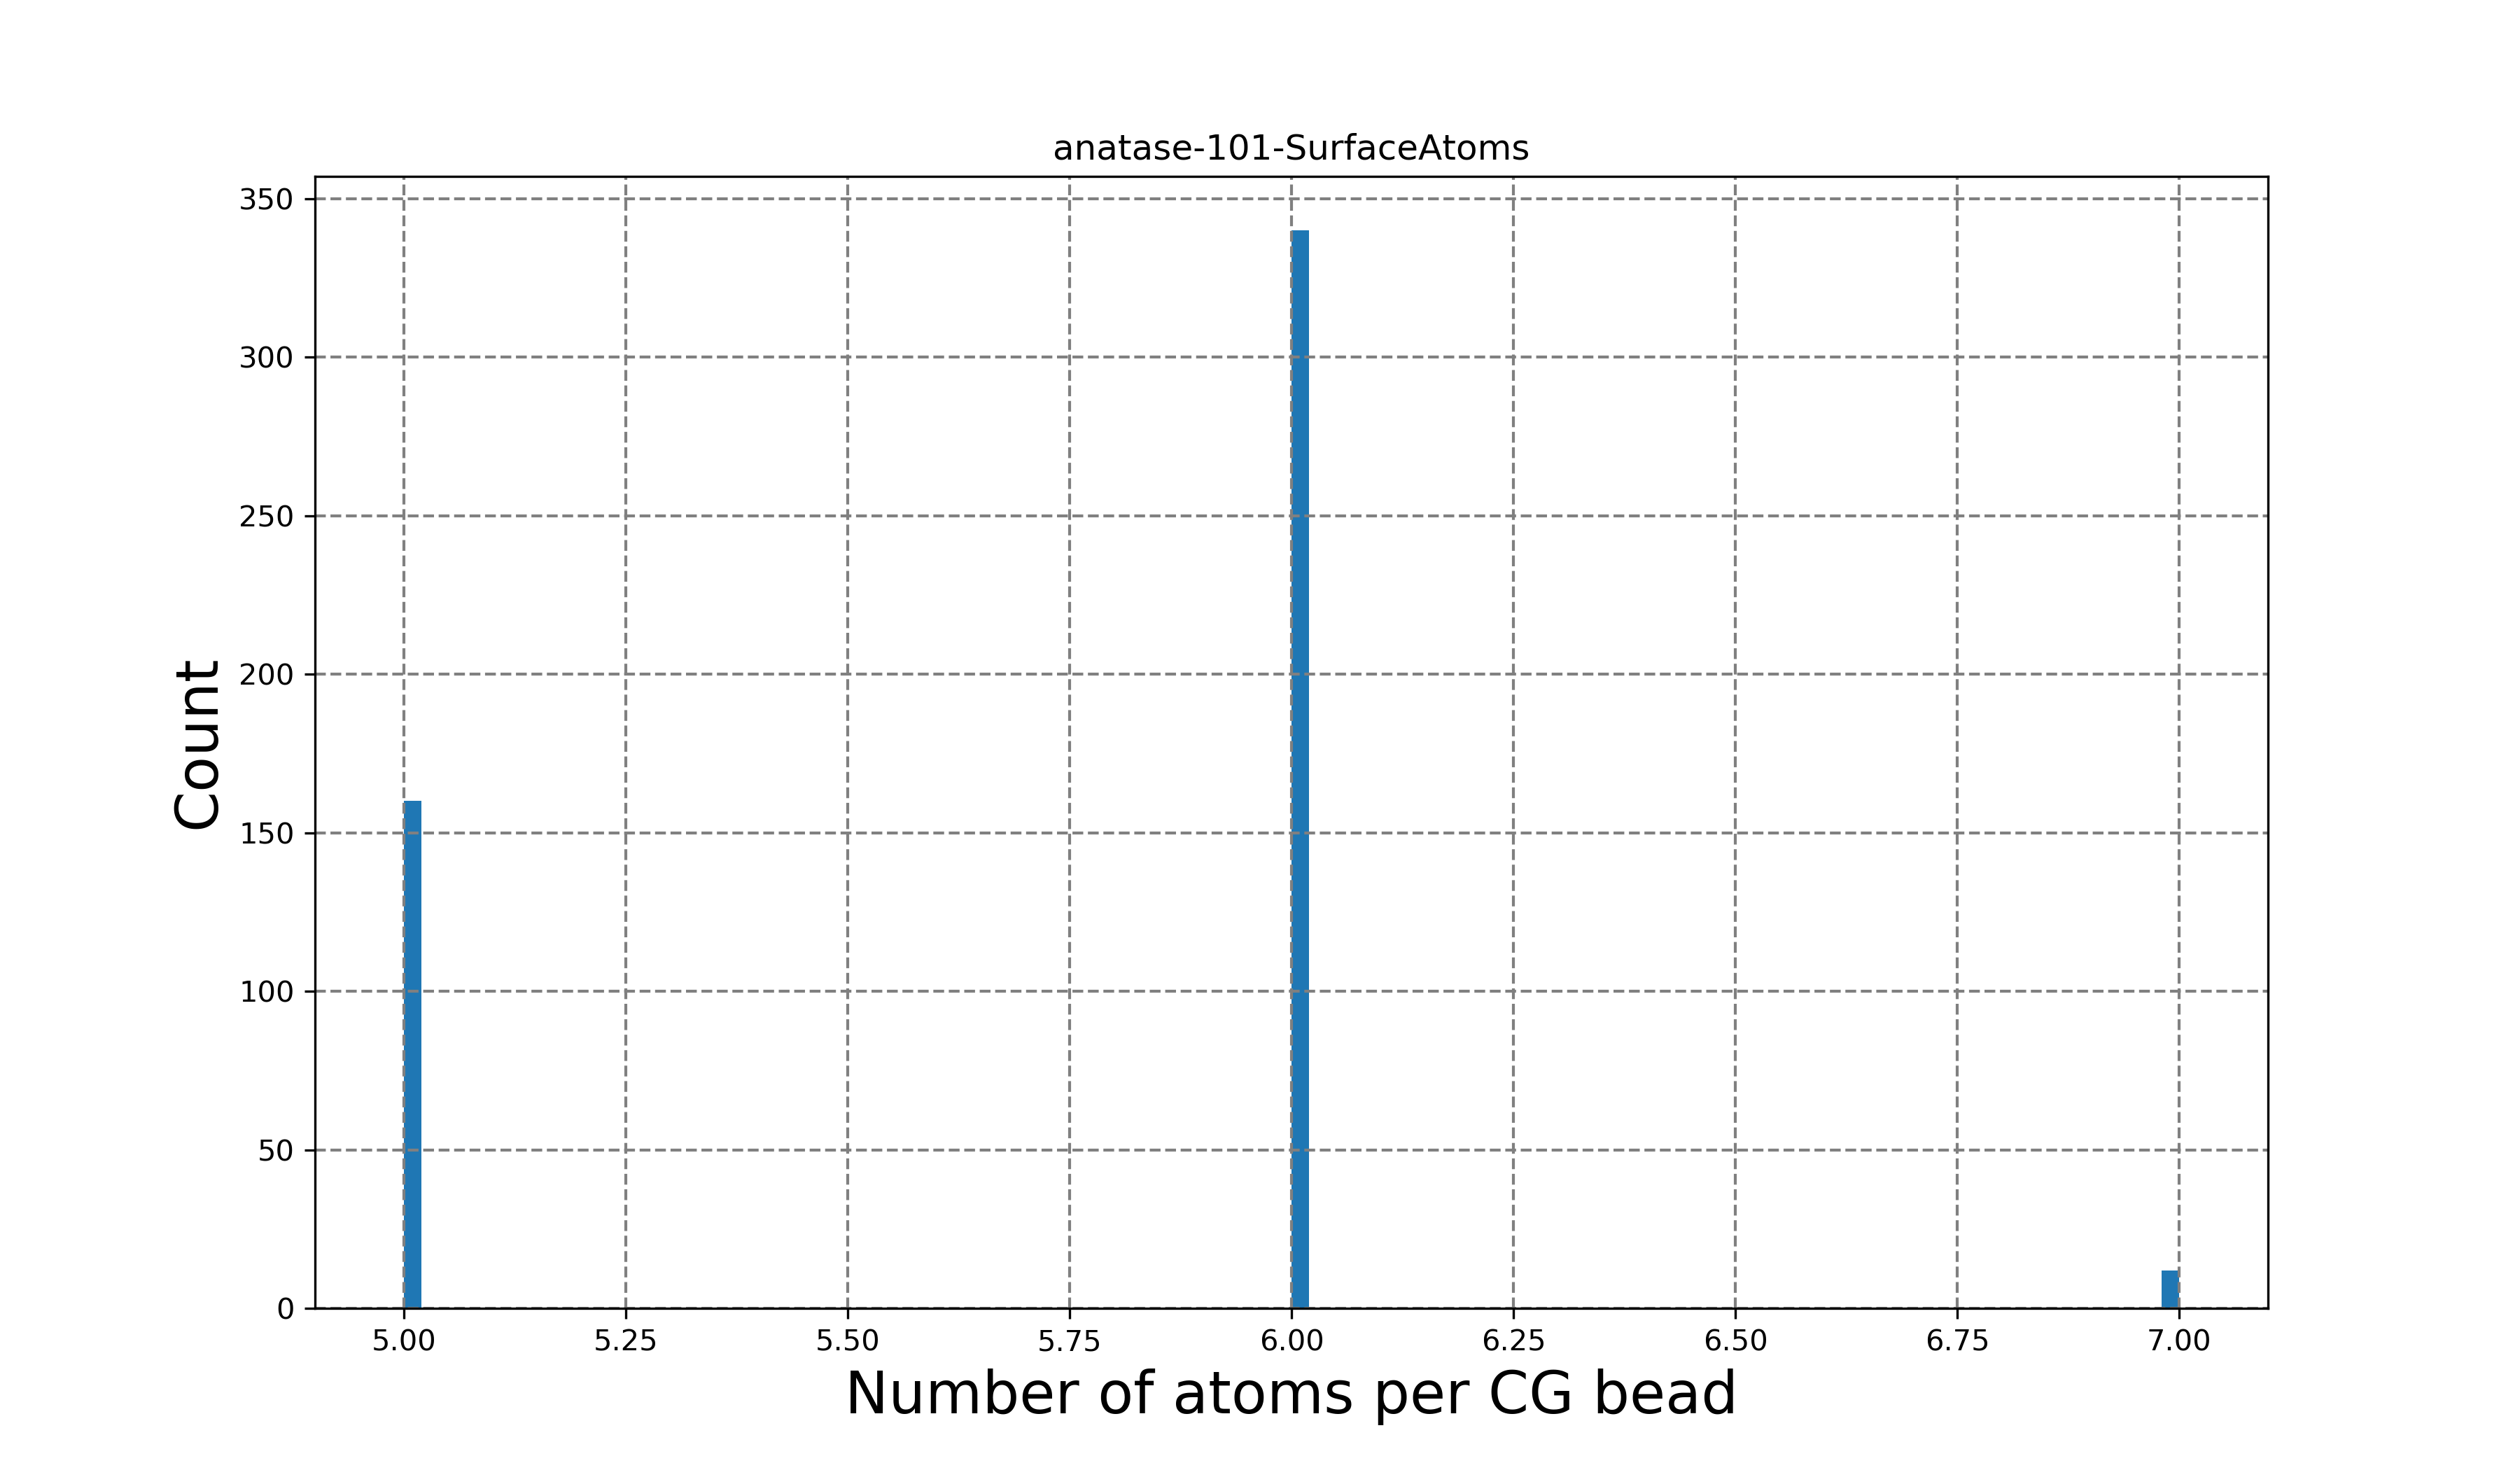
\includegraphics[scale=0.3]{anatase-101-SurfaceAtoms.png}
\caption{Distribution of assigned atoms for surface CG beads \textbf{after} fixing.}
\label{fig: anatase-101 histogram}
\end{figure}

It is clear that the distribution is much more uniform after fixing. 

Figure \ref{fig: representations} shows the atomistic model of anatase slab and the coarse-grained representation of the surface coarse-grained beads using the bead mapping scheme obtained with this program.

\begin{figure}[h]
\centering
\includegraphics[width=145mm]{Project-overview.png}
\caption{Atomic and CG representations of anatase slab.}
\label{fig: representations}
\end{figure}

\newpage
\section{Conclusion}
The \texttt{SlabCGBeadMapping.py} program enables automatic coarse-grained bead mapping of rectangular slabs. It was shown that the program can generate the bead mapping scheme for anatase slab with almost uniform distribution of atoms in the CG beads. In the future the program will be used to generate bead mapping scheme for other types of slabs and the support for bead mapping of spherical nanoparticles will be added.

\end{document}